\section{Discussion}

\noindent 
{\bf Information Flow Invariants.~}
We need to caution that any reactive system cannot
be provably secure. 

CloudFlow enacts a best-effort approach that aims to minimize the
vulnerability window during which an attack can be mounted against a target
VM.  In practice however, we observe that the window of vulnerability is so
small (\textless 5ms, Section \ref{sec:evaluation}) that it easily defeats any
existing and foreseeable side-channel attacks which are usually low-bandwidth
and require comparatively ample amount of time to deploy \cite{SideCrypto,SideCloud,PrimeProbe12}
(\textgreater hours).

\noindent
{\bf Users \& Groups.~}
%
CloudFlow allows the straightforward definition and enforcement of user and
group/role-based policies. Roles can be associated with underlying SELinux
labels which can then be used in the policy definitions. 

\noindent
{\bf Centralizing Policy Management.~}
%
Currently CloudFlow is using a database attached to OpenStack as a Policy
Store.  Whenever a particular VM is being launched, it needs to also attach
all policies pertaining to the launch request to be propagated along with its VM launch
request.  The target VM host thus only needs to keep track of policies that
are locally relevant.  This significantly reduces the complexity of policy
checking required by the local PolicyD instance and reduces latency for
migration decisions.

The process can be further streamlined by ensuring a default automatic
OpenStack-driven policy-to-VM mapping and propagation that can determine
applicable policies from the user's session credentials. However, the
existence of a set of cloud-wide policy repositories from
which users can chose individual subsets of policies of interest may be desirable. 

Finally, the policy management system would benefit from a (partial)
ordering of runtime labels.  This would enable streamlined conflict
resolution, e.g., a policy may specify that the ``lower'' labeled VM
should be migrated in the case of triggered inter-VM policy conflicts.

%cloudflow is for security
%you can use it for management
%policies can be geared towards management rather than security in order to provide segregation at the node level
%no need for centralized management as each role manages its own policies independently

\noindent
{\bf Management \& Scheduling~}
%
Even though CloudFlow is primarily a security tool, the design allows for fine-grained management-oriented usage. The policy engine is oblivious to the semantics of the policies and labels. Policies can be used to describe arbitrary segregations of the in-house cloud in terms of users, workloads and resources. E.g. a CPU intensive workload can be tagged with a corresponding 'CPU-intensive' label. Further VMs with this label are only allowed to migrate to machines that can handle more CPU cycles but may be lacking in storage or other resources. Machines can simply be labeled by tagging custom users or tasks with desired performance numbers for policy usage. Here policy 'conflicts' can be described in terms of performance rather than security. This produces a self-scheduling cloud as VMs automatically end up in places that make sense in terms of real-time resource usage. This kind of scheduling allows VMs to relocate only when needed. VMs can switch between CPU-intensive or I/O-intensive tasks triggering label changes and get scheduled on appropriate nodes transparently.

\begin{figure}[t]
\begin{center}
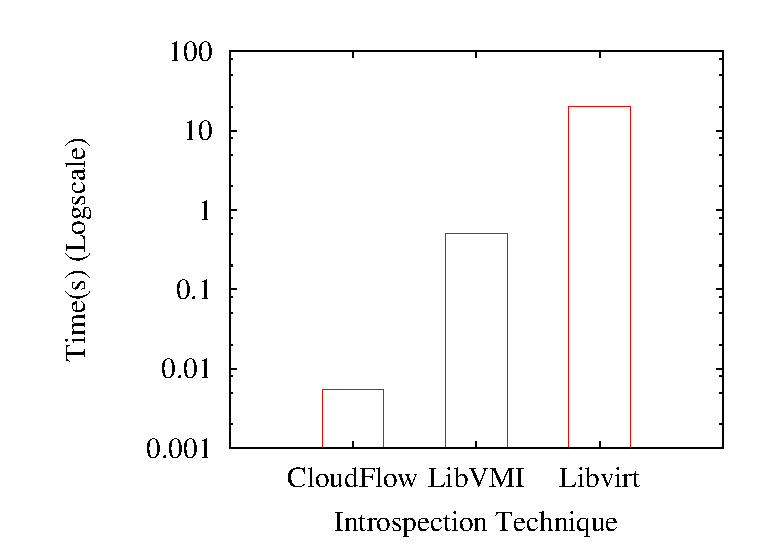
\includegraphics[scale=0.6]{figures/introspectionwindow.eps}
%\vspace{30pt}
\caption{\small 
%
CloudFlow features a low impact introspection design that allows it to
perform significantly faster than existing introspection libraries.  The
shorter the introspection cycle, the smaller the window of vulnerability
during which a VM can be attacked.
% 
\label{cloudflow:figure:introspectionwindow}}
\end{center}
\end{figure}

\begin{figure}[t]
\begin{center}
\includegraphics[scale=0.6]{figures/guestslowdown.eps}
%\vspace{30pt}
\caption{\small 
%
CloudFlow has a minimal overhead, below 2\% slowdown in guest workloads. 
Performance slowdown caused by CloudFlow remains well within the normal
variation shown by typical workloads, represented here by the error bars. 
%
\label{cloudflow:figure:guestslowdown}}
\end{center}
\end{figure}


